% !TeX spellcheck = en_US
\chapter{Decentralized system}\label{cha:decentralizedSystem}

\section{Platform}

\section{DDS configuration}

\section{Algorithm}\label{sec:algoDecen}

\begin{tikzpicture} 
\begin{umlseqdiag} 
\umldatabase{DB} 
\umlmulti{DataSimulator}
\umlmulti{Regulation Controller}
\umlmulti{Monitor}
\begin{umlcall}[op=getAlldata(), type=asynchron, return=0]{DB}{DataSimulator}
\begin{umlfragment}[type=ForAll, label=Samples, inner xsep=8, fill=white!10]
\begin{umlcall}[op=Simumlation data, type=synchron, return=setpoint]{DataSimulator}{Regulation Controller}

\end{umlcall}
\begin{umlfragment}[type=opt, fill=white!10]
\begin{umlcall}[op=UpdateUI(), type=asynchron, return=0]{DataSimulator}{Monitor}
\end{umlcall}
\end{umlfragment}
\end{umlfragment}

\begin{umlcall}[op=saveData(), type=asynchron, return=0]{DataSimulator}{DB}
\end{umlcall}	
\end{umlcall}

\end{umlseqdiag} 
\end{tikzpicture}

\includegraphics{figures/metapost/ClassDiagramHPPP.1}

\section{Graphical Interface} \label{sec:graphicalInterface}
In order to visualize the system a graphical user interface has been constructed using Matlab, Simulink and DDS Blockset for Simulink.
These tools combined allows the creation of a Simulink model which taps into the communication of the DDS framework.
The data collected from via the Simulink model can then be transferred to Matlab for further processing or visualization.

The main objective of the graphical interface is to visualize what messages is currently flowing in the system but almost as important is the ability to collect data for further analysis.
Matlab is a powerful tool for anlysis and having the data transferred live from the DDS framework to matlab allows for both live as well as in depth analysis on a dataset collected during an experiment.

Currently only the decentralized system can be visualized and controlled using the graphical interface. Given the scope and focus of this thesis the value added by visualizing the centralised system would be minimal. Both the decentralized and centralized system can log data using the Simulink models.

\subsection{DDS Blockset for Simulink}
RTI has created a Blockset for Simulink allowing a Simulink model to interact with the DDS Participant and other entities in a DDS enabled network.
The blockset consists of a toolbox containing 6 blocks. Common for all blocks except the DDS Time block is that they can be configured with a default or custom Quality of Service profile as well as a sample time. The Quality of Service profile must match the profile used in the network you want to participate in. The sample time is related to the Simulink model and specifies the timeinterval between samples.

\begin{figure}[h]
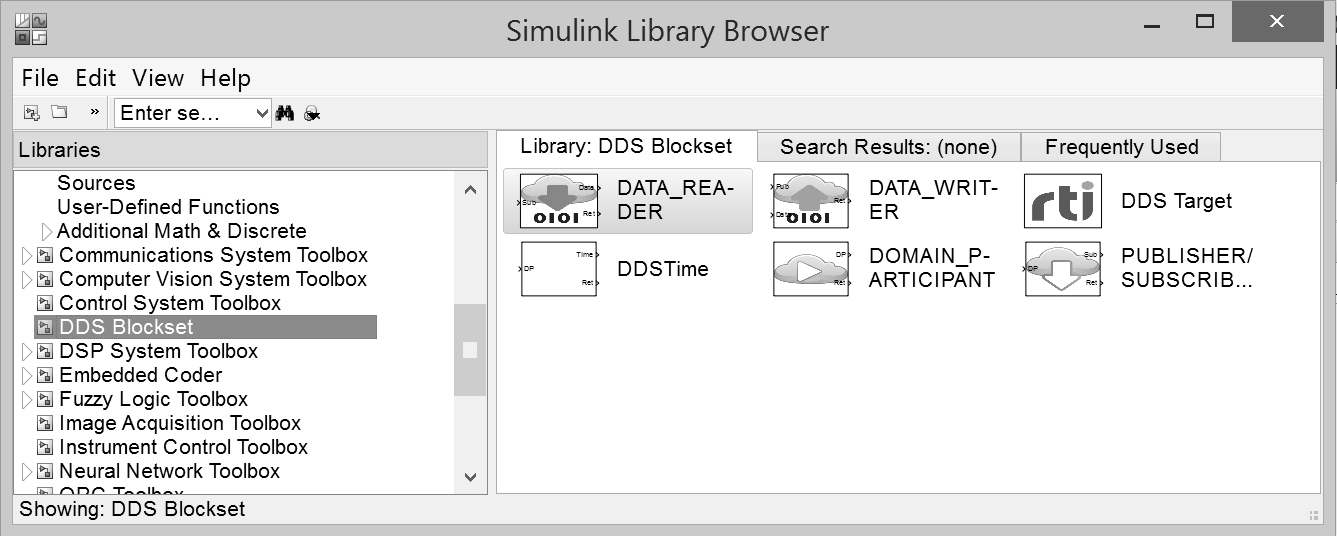
\includegraphics[width=\textwidth]{figures/DDSBlockset}
\captionsetup{format=plain,font=footnotesize,labelfont={bf,defaultCapFont},labelsep=quad,singlelinecheck=no}
	\caption[DDSBlockset blocks for Simulink]{
		\label{fig:DDSBlocksetBlocks} 
		\footnotesize{%
			DDSBlockset blocks for Simulink.
		}
	}
\end{figure}


\paragraph{The DomainParticipant block} is the equivalent to the DomainParticipant entity in DDS. This block allows for configuration of the DomainID which links the DomainParticipant to a specific DDS domain.

\paragraph{The Publisher/Subscriber block} can be configured as either a Publisher or a Subscriber and will act as either based on the chosen configuration.

\paragraph{The DataWriter block} is the equivalent to the DataWriter entity in DDS. This block can write data to a topic in DDS. The DataWriter block must be configured with the name of the Topic as well as the name of the Topic Type created by the Simulink Bus that is input to the DataWriter.

\paragraph{The DataReader block} is the equivalent to the DataReader entity in DDS. This block can read data from a topic in DDS. The DataReader block must be configured with the name of the Topic as well as the name of the Topic Type created by the Simulink Bus that is input to the DataReader. The DataReader block can also be configured to either use Read() or Take() for obtaining the DDS data. The Read() command will leave the data in DDS memory, the Take() command will remove the data from DDS memory. The DataReader block is able to either poll DDS for data or wait for data until data is ready or a timeout occurs.

\paragraph{The DDSTarget block} is controls code generated for the DDS blocks in the Simulink model. It is possible to configure which version of DDS code will be generated for, either RTI Connext DDS(default), or RTI Connext Micro DDS. The type system can be configured to either static or dynamic as well as the discovery mode.

\paragraph{The Time block} can return the current time from DDS output in seconds and nanoseconds.

\subsection{Installation of DDS Blockset for Simulink}
To install DDS Blockset for Simulink follow the steps provided by Mathworks \cite{DDSBlocksetPilotSupportPackageUserGuide}. The installation is short but as described below additional work had to be done in order to make DDS Blockset for Simulink work properly with Matlab and Interface Definition Language files.

The problems described in the section all relates to installation of DDS Blockset for Simulink using Matlab 2013b on a Windows 8.1 x64 environment.
Other environments may be more or less optimal but have not been tested during this thesis.

There are a few caveats to be avoided when installing DDS Blockset for Simulink on Windows.
After installation of DDSBlockset for Simulink completes make sure the NDDSHOME path variable is set to C:\textbackslash Program Files(x86)\textbackslash RTI.
Notice that this path is different from the default path recommended by RTI which is C:\textbackslash Program Files(x86)\textbackslash RTI\textbackslash ndds.5.0.0 (version numbers may change).

DDS Blockset for Simulink has an import feature available for import of Interface Definition Language files. The import process creates a Simulink bus that the Simulink model can hook into and pull data from. In order to enable import of Interface Definition Language files additional setup must be performed.
Since Matlab does not provide a compiler fro C++ on x64 systems one must be downloaded. Microsoft provides a compiler in the Microsoft Windows SDK 7.1. Matlab must be told to use the compiler by using the mex -setup command. Finally the location of the binaries and the libraries that is downloaded with the new compiler must be added to path.

\subsection{Simulink model of the decentralized system}\label{subsec:decentralizedmodel}

\begin{figure}[b]
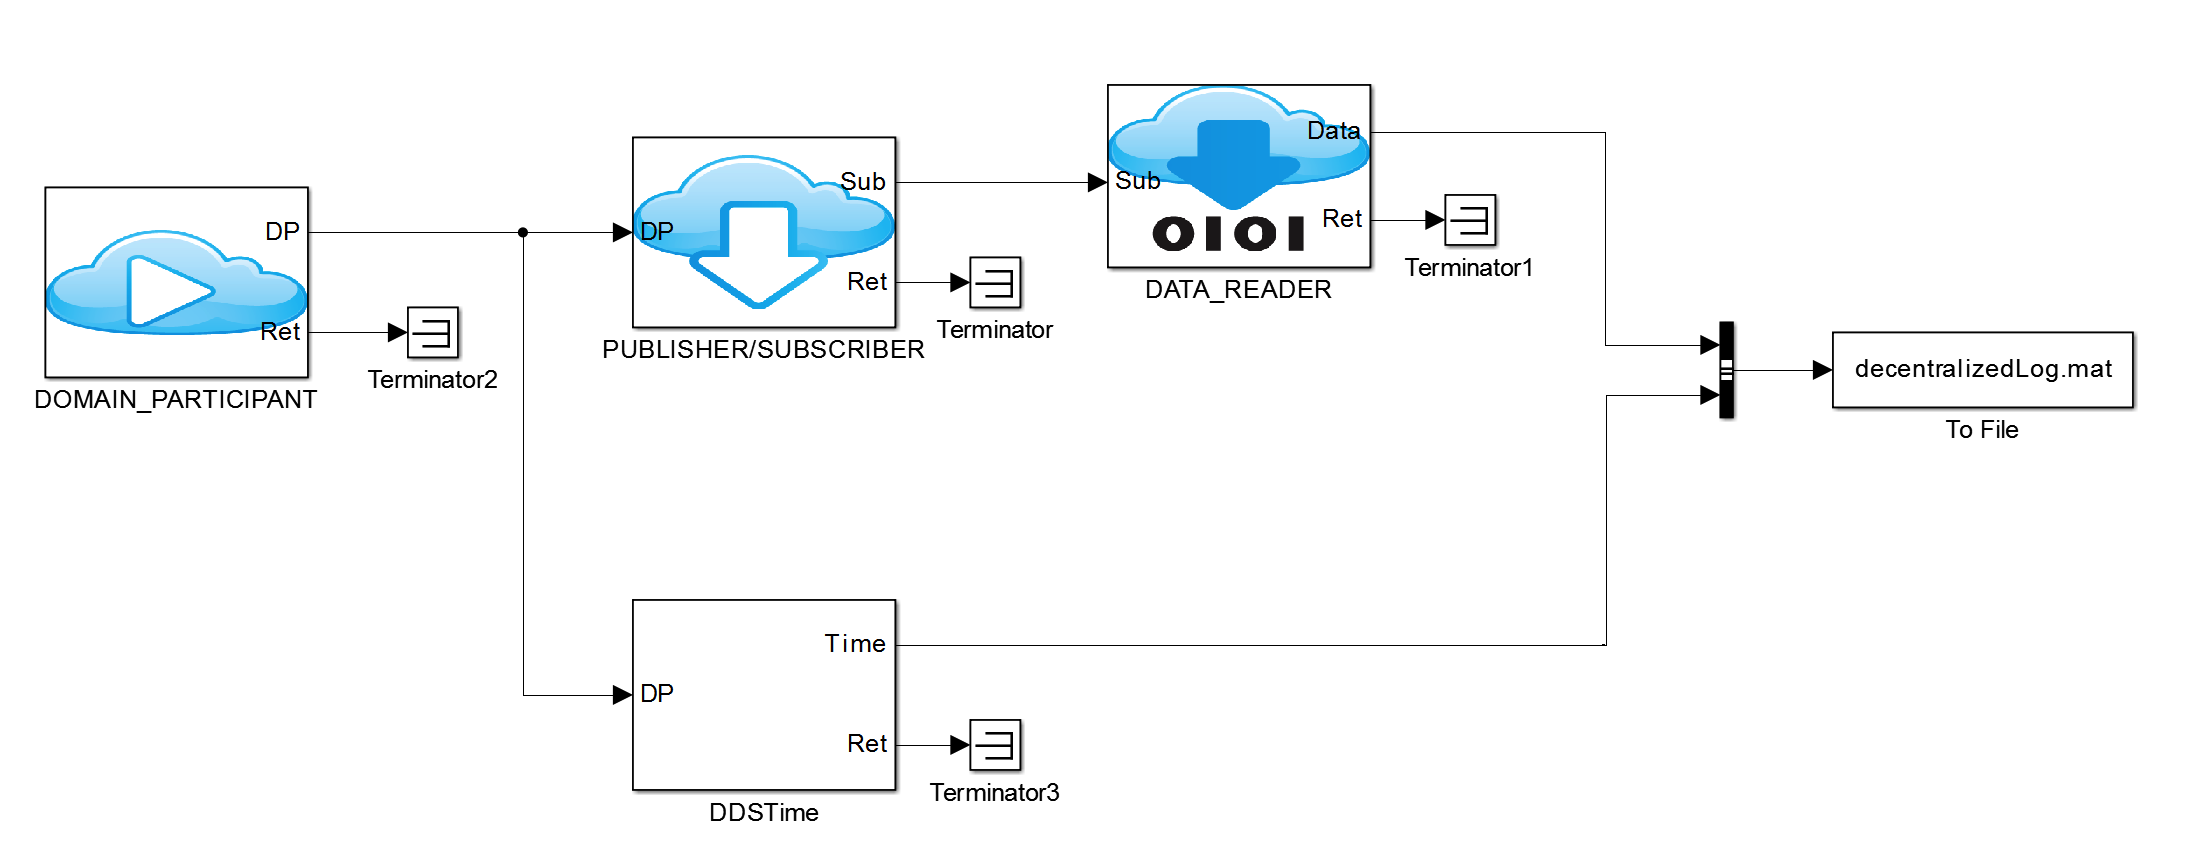
\includegraphics[width=\textwidth]{figures/DecentralizedModel}
\captionsetup{format=plain,font=footnotesize,labelfont={bf,defaultCapFont},labelsep=quad,singlelinecheck=no}
	\caption[Decentralized Simulink model]{
		\label{fig:decentralizedSimulinkModel} 
		\footnotesize{%
			Decentralized Simulink model.
		}
	}
\end{figure}

The Simulink model of the decentralized system is simple. The decentralized Simulink model has a DomainParticipant block in order to be able to receive data from the same domain as the turbines. It also has a Time block to enable logging and graphing of the current DDS time. Since the decentralized system only uses one DDS message type, TurbineMessage \{INSERT REFERENCE\}, to communicate between all the turbines in the system, the decentralized Simulink model has only one Subscriber block and one DataReader block. The Subscriber block specifies the topic to subscribe to and the DataReader block receives events every time a new TurbineMessage is available. The TurbineMessage that is received is logged to a .mat file together with the current DDS time for later use.

In order to transfer data from the Simulink model to Matlab eventlisteners must be implemented in a Matlab .m file. In the decentralized system the eventhandler listens for incoming events on the bus object that receives new data from the DataReader block. When new data is received the event fires and data can be collected from the Simulink model. Furthermore model execution can be controlled from Matlab, as well as parameters like model runtime.

\subsection{Simulink model of the centralized system}\label{subsec:centralizedmodel}
The Simulink model of the centralized system is a bit more complex. The centralized system contains three different messagetypes, TurbineDataMessage, RequestMessage, SetpointMessage, \{INSERT REFRENCE\} that all run on different topics. Because of this the centralized Simulink model contains one DomainParticipant, three Subscribers, one for each topic, and three DataReaders, one for each message type, in order to capture the communication in the centralized system. Every message received is logged to a .mat file together with the current DDS time.

\begin{figure}[h]
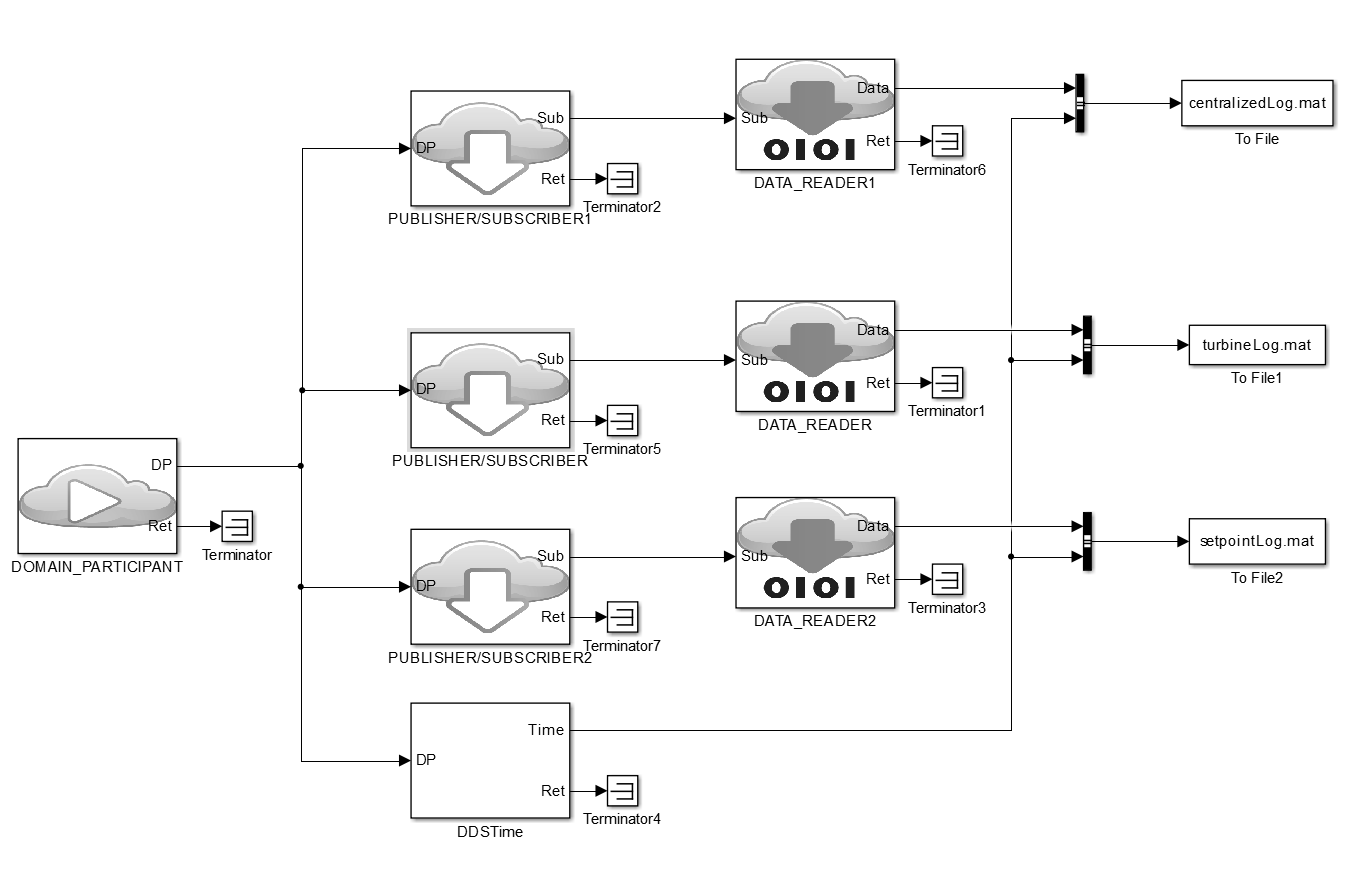
\includegraphics[width=\textwidth]{figures/CentralizedModel}
\captionsetup{format=plain,font=footnotesize,labelfont={bf,defaultCapFont},labelsep=quad,singlelinecheck=no}
	\caption[Centralized Simulink model]{
		\label{fig:centralizedSimulinkModel} 
		\footnotesize{%
			Centralized Simulink model.
		}
	}
\end{figure}